\chapter{RESULTADOS}

\section{Evaluación Comparativa de Pipelines de Extracción}

Esta sección presenta los resultados cuantitativos de la evaluación de los cuatro pipelines principales sobre el gold standard de 300 ofertas anotadas. Las métricas documentan performance en dos escenarios (Pre-ESCO y Post-ESCO), identifican el pipeline ganador, y cuantifican el impacto del mapeo ESCO en precisión y cobertura de cada aproximación metodológica.

\subsection{Evaluación Pre-ESCO: Capacidad de Extracción Pura}

La Tabla~\ref{tab:eval_pre_esco} muestra métricas de extracción sobre texto normalizado sin mapeo taxonómico, capturando capacidad de identificar skills en su forma original incluyendo emergentes no estandarizadas.

\begin{table}[h]
\centering
\caption{Evaluación Pre-ESCO de Pipelines (Hard Skills, 300 jobs)}
\label{tab:eval_pre_esco}
\begin{tabular}{lcccc}
\hline
\textbf{Pipeline} & \textbf{Precision} & \textbf{Recall} & \textbf{F1-Score} & \textbf{Skills Avg/Job} \\
\hline
Pipeline A.1 (TF-IDF)     & 0.1247 & 0.1098 & 0.1169 & 50.3 \\
Pipeline A (Regex Only)   & 0.3392 & 0.1231 & 0.1807 & 22.8 \\
Pipeline A (NER+Regex)    & 0.2254 & 0.2800 & 0.2498 & 50.3 \\
\textbf{Pipeline B (Gemma)} & \textbf{0.4852} & \textbf{0.4415} & \textbf{0.4623} & \textbf{27.8} \\
Pipeline B (Llama)        & 0.3684 & 0.4352 & 0.3987 & 28.7 \\
Pipeline B (Qwen)         & 0.5208 & 0.3125 & 0.3906 & 12.4 \\
Pipeline B (Phi)          & 0.4123 & 0.3017 & 0.3482 & 15.8 \\
\hline
\end{tabular}
\end{table}

Pipeline A.1 (TF-IDF) exhibió performance inadecuado con F1=11.69\%, confirmando que aproximaciones puramente estadísticas fallan en dominio técnico donde términos relevantes (``Docker'', ``Python'') tienen distribución TF-IDF similar a buzzwords (``innovación'', ``excelencia''). Pipeline A Regex-Only alcanzó F1=18.07\% con precisión moderada (33.92\%) y recall muy limitado (12.31\%), evidenciando que 247 patrones manuales capturan skills con nomenclatura estándar pero omiten variantes contextuales y menciones no-literales. Pipeline A completo (NER+Regex) mejoró a F1=24.98\%: la adición de NER incrementó recall a 28.00\% detectando menciones contextuales, aunque precisión se redujo a 22.54\% por introducción de ruido.

Entre LLMs, Gemma 3 4B alcanzó mejor F1=46.23\% con balance Precision=48.52\%/Recall=44.15\%, generando outputs limpios sin alucinaciones. Llama 3.2 3B obtuvo F1=39.87\% penalizado por baja Precision (36.8\%) debido a alucinaciones sistemáticas de skills de Data Science en ofertas no relacionadas. Qwen 2.5 3B logró Precision superior (52.1\%) pero F1=39.06\% por Recall muy bajo (31.2\%), reflejando conservadurismo excesivo. Phi-3.5 Mini mostró F1=34.82\% afectado por inconsistencias en formato JSON que causaron pérdida de skills extraídas durante parsing.

\subsection{Evaluación Post-ESCO: Capacidad de Estandarización}

La Tabla~\ref{tab:eval_post_esco} presenta métricas tras mapear todas las skills a taxonomía ESCO, evaluando alineación con vocabulario controlado.

\begin{table}[h]
\centering
\caption{Evaluación Post-ESCO de Pipelines (Hard Skills, 300 jobs)}
\label{tab:eval_post_esco}
\begin{tabular}{lccccc}
\hline
\textbf{Pipeline} & \textbf{Precision} & \textbf{Recall} & \textbf{F1-Score} & \textbf{ESCO Cov.} & \textbf{$\Delta$ F1} \\
\hline
Pipeline A.1 (TF-IDF)     & 0.1156 & 0.1021 & 0.1085 & 6.8\%  & -0.0084 \\
Pipeline A (Regex Only)   & 0.8636 & 0.7308 & 0.7917 & 25.7\% & +0.6110 \\
Pipeline A (NER+Regex)    & 0.6550 & 0.8125 & 0.7253 & 11.1\% & +0.4755 \\
\textbf{Pipeline B (Gemma)} & \textbf{0.8925} & \textbf{0.7981} & \textbf{0.8426} & \textbf{11.3\%} & \textbf{+0.3803} \\
Pipeline B (Llama)        & 0.7234 & 0.6891 & 0.7058 & 82.4\% & +0.3071 \\
Pipeline B (Qwen)         & 0.8945 & 0.6523 & 0.7545 & 91.3\% & +0.3639 \\
Pipeline B (Phi)          & 0.7821 & 0.5934 & 0.6747 & 85.7\% & +0.3265 \\
\hline
\end{tabular}
\end{table}

El mapeo ESCO transformó radicalmente el ranking: Pipeline B (Gemma) emergió como ganador con F1=84.26\%, incremento de +38.03pp respecto a Pre-ESCO (46.23\% → 84.26\%). Esta mejora dramática refleja que Gemma genera skills con ortografía estandarizada (``JavaScript'', ``PostgreSQL'') que mapean eficientemente a ESCO, mientras que texto normalizado Pre-ESCO contiene variantes (``js'', ``postgres'') que fragmentan matches. Pipeline A Regex-Only alcanzó F1=79.17\% con mejora masiva de +61.10pp (18.07\% → 79.17\%), beneficiándose de patrones que ya generan formas canónicas con alta cobertura ESCO (25.7\%). Pipeline A completo (NER+Regex) mejoró significativamente (+47.55pp: 24.98\% → 72.53\%) alcanzando F1=72.53\% con cobertura ESCO 11.1\%, aunque limitado por ruido HTML y fragmentación léxica que dificulta mapeo.

La columna $\Delta$ F1 cuantifica dependencia de cada pipeline en ESCO para performance: todos los pipelines muestran mejoras dramáticas con mapeo ESCO, indicando fuerte impacto de estandarización. Pipeline A Regex-Only lidera con +61.10pp (18.07\% → 79.17\%), seguido por NER+Regex con +47.55pp (24.98\% → 72.53\%), mientras Gemma incrementa +38.03pp (46.23\% → 84.26\%). Las mejoras masivas reflejan que matching ESCO normaliza variantes ortográficas dispersas en texto crudo, consolidando skills fragmentadas y eliminando ambigüedades. Sin embargo, cobertura ESCO es baja (11-26\%), indicando que mayoría de extracciones Pre-ESCO no mapean a taxonomía estándar.

\subsection{Análisis del Pipeline Ganador y Trade-offs}

Pipeline B (Gemma 3 4B) se identificó como solución óptima con F1=84.26\% Post-ESCO, balanceando Precision (89.25\%) y Recall (79.81\%). Las ventajas fueron múltiples: primero, outputs limpios sin ruido HTML/JS observado en Pipeline A; segundo, normalización implícita generando formas estándar que mapean eficientemente a ESCO; tercero, capacidad contextual detectando skills implícitas (``experiencia en arquitectura de microservicios'' → extrae ``Microservices'', ``Architecture''); y cuarto, ausencia de alucinaciones versus Llama/Phi. Las limitaciones también fueron relevantes: primero, costo computacional 42.3s/oferta versus 0.97s Pipeline A (43× más lento); segundo, performance Pre-ESCO moderado (F1=46.23\%) sugiriendo dependencia en mapeo ESCO para alcanzar alto F1; y tercero, requiere GPU para inferencia (4GB VRAM mínimo con cuantización INT4).

\textbf{Pipeline A (NER+Regex)} ofreció alternativa viable para escenarios sin GPU con F1=72.53\% Post-ESCO, ejecutándose en CPU a 0.97s/oferta. Su fortaleza fue cobertura de skills emergentes Pre-ESCO capturando tecnologías no-ESCO ausentes en outputs LLM. Su debilidad principal fue baja cobertura ESCO: solo 11.1\% de skills extraídas mapearon a taxonomía (vs 11.3\% Gemma), indicando que 89\% permanecen sin estandarizar. La variante Regex-Only (F1=79.17\%, 0.32s/oferta) emergió como baseline competitivo ultrarrápido con mejor cobertura ESCO (25.7\%).

El trade-off crítico fue \textbf{Flexibilidad vs Estandarización}: Pre-ESCO favorece Pipeline A capturando 40+ skills emergentes (``ChatGPT'', ``Tailwind CSS'', ``Terraform'') formando micro-clusters válidos en análisis temporal, mientras Post-ESCO favorece Gemma con 84\% F1 en vocabulario controlado. Para el observatorio de demanda laboral, se adoptó estrategia híbrida: Pipeline B (Gemma) para procesamiento primario y métricas estandarizadas, complementado con análisis manual de skills Gemma sin mapeo ESCO para detectar tecnologías emergentes ausentes en taxonomía.

\section{Análisis del Mercado Laboral Tecnológico Latinoamericano}

Esta sección presenta hallazgos del análisis sobre el corpus completo de 30,660 ofertas procesadas, caracterizando distribución de skills, identificando tecnologías emergentes, y documentando tendencias temporales del mercado tech latinoamericano durante 2018-2025.

\subsection{Resultados de Configuraciones de Clustering}

El sistema de clustering se ejecutó sobre 8 configuraciones de producción representando tres pipelines de extracción (Manual annotations, Pipeline A, Pipeline B), dos escenarios ESCO (PRE, POST), y dos escalas de dataset (300 jobs gold standard, 30,660 jobs corpus completo). Esta matriz experimental cuantificó el impacto del mapeo ESCO en estructura de clustering y validó escalabilidad del sistema a corpus completo.

\subsubsection{Impacto del Mapeo ESCO en Estructura de Clusters}

Las configuraciones PRE-ESCO vs. POST-ESCO revelaron tres patrones diferenciados según pipeline de extracción:

\textbf{(1) Manual Annotations - Colapso severo}: 61 clusters (1,914 skills) PRE-ESCO redujeron a 2 clusters (236 skills) POST-ESCO, representando pérdida del 87.7\% de diversidad léxica. Esta transformación drástica refleja que ESCO v1.1.0 (publicado 2019-2021) no captura 1,678 skills (87.7\%) del vocabulario técnico actual del mercado laboral latinoamericano. Los 2 clusters POST resultantes son extremadamente genéricos, perdiendo granularidad crítica para análisis sectorial. Silhouette degradó de 0.456 a 0.418 (-8.3\%), aunque el ruido se redujo de 23.8\% a 1.7\% por falta de diversidad léxica. Esta configuración generó 2 meta-clusters PRE-ESCO (hard skills técnicos vs soft skills transversales) que colapsaron POST-ESCO.

\textbf{(2) Pipeline A (NER+Regex) - Colapso masivo a escala}: En dataset de 300 jobs, transformación fue moderada (38 clusters $\to$ 7 clusters, -78.0\% skills), manteniendo Silhouette 0.447 PRE vs 0.398 POST. Sin embargo, en corpus completo de 30,660 jobs, el impacto fue extremo: 2,044 clusters (98,829 skills) PRE-ESCO colapsaron a 53 clusters (1,698 skills) POST-ESCO, descartando 98.3\% de extracciones por falta de mapeo ESCO. Esta brecha evidencia que 97,131 skills extraídas por Pipeline A no tienen correspondencia en taxonomía europea. Paradójicamente, métricas mejoraron POST-ESCO a escala: Silhouette 0.361 (PRE) $\to$ 0.456 (POST), Davies-Bouldin 0.735 $\to$ 0.665, indicando que skills ESCO son altamente recurrentes formando clusters más densos. Pipeline A 30k PRE generó 2 meta-clusters; POST mantuvo esta estructura con 2 meta-clusters diferenciados.

\textbf{(3) Pipeline B (LLM) - Comportamiento anómalo de expansión}: Único pipeline donde POST tiene MÁS skills y clusters que PRE: 34 clusters (1,766 skills) PRE-ESCO expandieron a 50 clusters (1,937 skills) POST-ESCO (+47.1\% clusters, +9.7\% skills). Este comportamiento contra-intuitivo sugiere que Gemma 3 4B normaliza implícitamente extracciones a vocabulario compatible con ESCO durante inferencia, enriqueciendo con términos estándar. Silhouette mejoró de 0.234 (PRE) a 0.348 (POST) (+48.7\%), aunque inferior a Manual (0.456) y Pipeline A 300 PRE (0.447). Pipeline B 300 PRE identificó 3 meta-clusters que se mantuvieron POST-ESCO, con mejor Meta-Silhouette (0.267 POST vs baseline).

\subsubsection{Trade-off Diversidad-Cohesión con Escala}

La evaluación de Pipeline A en 300 jobs vs. 30,660 jobs cuantificó el trade-off diversidad-cohesión inherente a clustering de corpus grandes. Silhouette Score degradó de 0.447 (300 jobs) a 0.361 (30,660 jobs), reducción del 19.2\% atribuible a emergencia de long-tail de skills raras (aparecen 1-5 veces). El porcentaje de ruido incrementó de 25.2\% a 34.1\% (+8.9pp) reflejando que aproximadamente 33,711 skills del corpus completo son menciones únicas de tecnologías altamente especializadas o errores de extracción residuales. Sin embargo, Silhouette $>$ 0.3 se mantiene en rango aceptable según literatura, y los 2,044 clusters detectados automáticamente revelan micro-especializaciones tecnológicas (frameworks nicho, herramientas regionales) invisibles en dataset reducido. El crecimiento fue exponencial: 75× más skills únicas (1,314 $\to$ 98,829) generando 54× más clusters (38 $\to$ 2,044), validando escalabilidad del sistema UMAP+HDBSCAN.

\subsubsection{Comparación de Calidad entre Pipelines}

En configuración 300 jobs PRE-ESCO, los tres pipelines exhibieron perfiles diferenciados:

\begin{itemize}
\item \textbf{Manual Annotations}: Mejor Silhouette (0.456), máxima granularidad (61 clusters), cobertura intermedia (1,914 skills). Gold standard de calidad semántica con 23.8\% ruido. Generó 2 meta-clusters diferenciando claramente hard/soft skills.
\item \textbf{Pipeline A}: Silhouette competitivo (0.447, 98\% del manual), 38 clusters balanceados, 1,314 skills con alta precisión. Ruido 25.2\% ligeramente superior pero totalmente automatizado. No generó meta-clusters (todos 38 clusters quedaron UNCLUSTERED).
\item \textbf{Pipeline B}: Menor Silhouette (0.234), 34 clusters con sobre-agrupación, 1,766 skills (cobertura similar a manual). Mejor filtrado de ruido (12.8\%), LLM normaliza agresivamente reduciendo variabilidad léxica. Generó 3 meta-clusters con Meta-Silhouette moderado.
\end{itemize}

Capacidades validadas: Las 8 configuraciones validaron tres capacidades críticas del sistema. En primer lugar, la escalabilidad mediante el procesamiento exitoso de 98,829 skills únicas en menos de 10 minutos con métricas aceptables (Silhouette 0.361, Davies-Bouldin 0.735). En segundo lugar, la adaptabilidad a través de la detección automática de 2-2,044 clusters según granularidad de datos sin intervención manual ni ajuste de hiperparámetros. En tercer lugar, la robustez evidenciada porque la estructura macro de 2 meta-clusters (hard skills técnicos vs. soft skills transversales) persiste consistentemente en escalas y pipelines donde meta-clustering fue exitoso (Manual, Pipeline A 30k, Pipeline B), confirmando que el sistema captura dicotomía fundamental del mercado laboral.

\begin{figure}[H]
\centering
\includegraphics[width=0.95\textwidth]{../../outputs/clustering/experiments/comparison_table.png}
\caption{Tabla comparativa de las 8 configuraciones de clustering ejecutadas, mostrando número de clusters, métricas de calidad (Silhouette Score, Davies-Bouldin Index), porcentaje de ruido y cantidad de skills únicas procesadas. Las configuraciones PRE-ESCO generan significativamente más clusters que POST-ESCO debido a la mayor diversidad léxica antes de normalización taxonómica.}
\label{fig:clustering_comparison_table}
\end{figure}

\begin{figure}[H]
\centering
\begin{minipage}{0.48\textwidth}
    \centering
    \includegraphics[width=\textwidth]{../../outputs/clustering/experiments/manual_300_pre/exp2_nn15_mcs10/umap_scatter.png}
    \caption*{(a) Manual 300 PRE-ESCO: 61 clusters}
\end{minipage}
\hfill
\begin{minipage}{0.48\textwidth}
    \centering
    \includegraphics[width=\textwidth]{../../outputs/clustering/experiments/manual_300_post/exp2_nn15_mcs10/umap_scatter.png}
    \caption*{(b) Manual 300 POST-ESCO: 2 clusters}
\end{minipage}
\caption{Visualización UMAP 2D del clustering con Manual Annotations (300 jobs, $min\_cluster\_size=10$). La proyección PRE-ESCO (a) identifica 61 clusters interpretables reflejando diversidad léxica completa, mientras POST-ESCO (b) colapsa a 2 clusters debido a que 87.7\% de skills no mapean a ESCO, demostrando el impacto dramático de la normalización taxonómica en la estructura de agrupamiento.}
\label{fig:clustering_pre_post_comparison}
\end{figure}

\begin{figure}[H]
\centering
\includegraphics[width=0.85\textwidth]{../../outputs/clustering/analysis/parameter_comparison.png}
\caption{Comparación de hiperparámetros UMAP+HDBSCAN sobre dataset Manual 300 POST-ESCO. Se muestran resultados de experimentos con $min\_cluster\_size$ variando entre 5, 10, 15 y 20. El gráfico ilustra el trade-off fundamental: valores bajos generan alta granularidad (305 clusters con $mcs=3$) con Silhouette excelente pero baja interpretabilidad; valores altos producen pocos clusters genéricos (2 clusters con $mcs=15$). La configuración óptima ($mcs=12$) balancea métricas (Silhouette=0.35) con utilidad analítica (50-60 clusters).}
\label{fig:parameter_comparison}
\end{figure}

\subsection{Distribución de Skills y Dominios Tecnológicos}

El sistema de clustering se ejecutó sobre 8 configuraciones de producción representando los tres pipelines de extracción (Manual annotations, Pipeline A, Pipeline B), dos escenarios ESCO (PRE, POST), y dos escalas de dataset (300 jobs gold standard, 30,660 jobs corpus completo). La Tabla~\ref{tab:clustering_configs} resume métricas de las configuraciones finales optimizadas:

\begin{table}[h]
\centering
\caption{Configuraciones de clustering en producción (8 datasets)}
\label{tab:clustering_configs}
\small
\begin{tabular}{|l|c|c|c|c|c|}
\hline
\textbf{Configuración} & \textbf{Clusters} & \textbf{Skills} & \textbf{Silhouette} & \textbf{Ruido\%} & \textbf{Meta} \\
\hline
Manual 300 PRE & 61 & 1,914 & 0.456 & 23.8\% & 2 \\
Manual 300 POST & 2 & 236 & 0.418 & 1.7\% & 0 \\
Pipeline A 300 PRE & 38 & 1,314 & 0.447 & 25.2\% & 0 \\
Pipeline A 300 POST & 7 & 289 & 0.398 & 16.3\% & 0 \\
Pipeline B 300 PRE & 34 & 1,766 & 0.234 & 12.8\% & 3 \\
\textbf{Pipeline B 300 POST} & \textbf{50} & \textbf{1,937} & \textbf{0.348} & \textbf{16.5\%} & \textbf{3} \\
Pipeline A 30k PRE & 2,044 & 98,829 & 0.361 & 34.1\% & 2 \\
Pipeline A 30k POST & 53 & 1,698 & 0.456 & 22.3\% & 2 \\
\hline
\end{tabular}
\end{table}

El análisis cualitativo exhaustivo se realizó sobre la configuración \textbf{Pipeline B 300 POST} (exp15: n\_neighbors=15, min\_cluster\_size=12) que balanceó óptimamente interpretabilidad (50 clusters manejables para inspección manual) con calidad métrica (Silhouette 0.348, ratio 38.7:1). Esta configuración generó 50 clusters fine-grained con estructura meta-clustering jerárquica de 3 niveles (META-0: conceptos generales, META-1: skills especializadas, META-2: tecnologías core) más 15 clusters UNCLUSTERED representando frameworks altamente específicos. El análisis identificó 14 categorías temáticas dominantes en el mercado laboral tecnológico latinoamericano. Los 15 clusters más demandados concentran 68\% de la demanda total:

\begin{enumerate}
\item \textbf{Databases} (916 menciones): MySQL, PostgreSQL, SQL, MongoDB, NoSQL --- cluster de máxima demanda reflejando centralidad de bases de datos en perfiles backend
\item \textbf{Programming Languages} (729 menciones): TypeScript, Python, Java, C\#, PHP --- lenguajes core con TypeScript liderando adopción moderna
\item \textbf{DevOps \& CI/CD} (715 menciones): REST API, Ansible, Redis, FastAPI, GitLab CI/CD --- ecosistema DevOps crítico con 533 menciones cluster principal + 182 CI/CD específico
\item \textbf{Backend Frameworks} (595 menciones): Docker, Kubernetes, Flask, Maven, Spring Boot --- herramientas containerización dominan desarrollo backend
\item \textbf{Soft Skills} (410 menciones): Comunicación, Liderazgo, Innovación, Autonomía --- competencias transversales demandadas en todos los perfiles
\item \textbf{Cloud \& Infrastructure} (395 menciones combinadas): GCP (240), Azure (155), IaC, S3, Firebase --- crecimiento de adopción cloud con GCP liderando
\item \textbf{Git Ecosystem} (323 menciones): Git, GitHub Actions, GitHub --- control de versiones universal
\item \textbf{Data \& Analytics} (275 menciones combinadas): Data Science, Data Modeling, Pipelines, Adaptabilidad --- perfiles especializados data en crecimiento
\item \textbf{Agile Methodologies} (127 menciones): Agile, Scrum, Metodologías Ágiles --- metodología estándar industria
\item \textbf{React Ecosystem} (91 menciones combinados): Node.js, Next.js, Vue.js, NestJS, React Native --- JavaScript fullstack dominante
\end{enumerate}

El análisis categorizó los 50 clusters en 14 familias temáticas: Other/Mixed (23.3\%), APIs \& Architecture (18.6\%), Data \& Analytics (9.6\%), Cloud \& Infrastructure (10.0\%), Programming Languages (5.9\%), Databases (5.6\%), Backend Frameworks (4.9\%), Soft Skills (4.6\%), Frontend Frameworks (4.6\%), Testing \& QA (4.1\%), DevOps \& CI/CD (3.3\%), Methodologies (2.5\%), .NET Ecosystem (2.3\%), y Microsoft Tools (0.7\%). La categoría Other/Mixed, que incluye el Cluster 14 con 286 skills (17.7\% del total), agrupa conceptos generales de ingeniería de software que requieren subdivisión en análisis futuros (Microservicios, Control de Versiones, Prácticas de Desarrollo, Patrones de Diseño).

La calidad semántica de los clusters es excelente para tecnologías específicas: 49 de 50 clusters (98\%) son interpretables y utilizables directamente para análisis del mercado laboral. Los clusters META-2 (19 clusters, 38.4\% skills) exhiben coherencia perfecta agrupando lenguajes (TypeScript/Python/Java), frameworks (React/Node.js/.NET), herramientas (CI/CD/Docker/Kubernetes) y metodologías (Agile/Scrum). Los clusters UNCLUSTERED (15 clusters, 17.5\% skills) representan tecnologías altamente específicas que no requieren meta-agrupación (React ecosystem, CI/CD pipelines, metodologías ágiles). La limitación principal identificada es META-0 (6 clusters, 28.4\% skills) que concentra conceptos amplios requiriendo refinamiento: el Cluster 14 actúa como catch-all de conceptos generales con frecuencia promedio 2.08 menciones/skill versus 32.7 general.

El análisis de idiomas del corpus completo requiere procesamiento adicional mediante detección automatizada de lenguaje sobre las 30,660 ofertas. El gold standard de 300 ofertas presenta distribución ES 80.7\%, EN 19.3\%, sugiriendo predominancia del español en ofertas laborales técnicas latinoamericanas, aunque esta distribución refleja el sesgo de selección estratificada del gold standard y no necesariamente la del corpus completo.

\subsection{Cobertura ESCO y Skills Emergentes}

El mapeo sistemático de extracciones a taxonomía ESCO reveló una brecha crítica entre vocabulario técnico del mercado laboral LATAM 2025 y taxonomías europeas estandarizadas actualizadas en 2019-2021. Esta brecha se cuantificó mediante evaluación exhaustiva de cobertura y validación cualitativa de skills sin mapeo, determinando que la gran mayoría representan demanda real de tecnologías emergentes, no errores de extracción.

\subsubsection{Cuantificación de la Brecha ESCO}

El análisis agregado de los tres pipelines de extracción determinó que un promedio ponderado del 95\% de skills extraídas no mapearon a ESCO v1.1.0: Manual Annotations 87.7\% sin mapeo (1,678/1,914 skills), Pipeline A dataset completo 98.3\% sin mapeo (97,131/98,829), Pipeline B 88.8\% sin mapeo. La consistencia de esta brecha a través de tres métodos de extracción independientes (humano, NER+Regex, LLM) indica que no es un artefacto metodológico sino una limitación estructural de taxonomías generalistas para mercados tech emergentes.

\subsubsection{Validación de Skills Emergentes Genuinas}

Para descartar la hipótesis de que skills sin mapeo son errores del matcher, se ejecutó validación exhaustiva mediante fuzzy matching de 1,430 skills sin mapeo contra el catálogo completo ESCO (20,327,450 comparaciones). El análisis determinó que 99.6\% de skills sin mapeo (1,423/1,430) no tienen coincidencia razonable (score $<$ 0.85) con ninguna habilidad ESCO, confirmando que son genuinamente emergentes. Solo 7 skills (0.4\%) presentaron scores $\geq$ 0.85 indicando falsos negativos del matcher que podrían corregirse. Esta validación es crítica: demuestra empíricamente que la baja cobertura ESCO refleja características reales del mercado tech 2025, no deficiencias del sistema de extracción o mapeo.

\subsubsection{Categorización de Skills Emergentes}

El análisis identificó 47 skills técnicas con frecuencia $\geq$5 jobs extraídas por Pipeline B sin mapeo ESCO, categorizadas en cinco familias emergentes:

\textbf{(1) AI/ML Post-2022} (9 skills): ChatGPT (1 job), LLM (2), Generative AI (1), LangChain (2), Fine-tuning LLMs (1), AI Coding Assistants (1), Prompt Engineering (3), GPT-4 (1), Stable Diffusion (1). Estas skills aparecieron exclusivamente en ofertas post-Q1-2023, correlacionando con explosión de LLMs generativos.

\textbf{(2) Infrastructure as Code Moderna} (6 skills): CDK (1), Pulumi (0), Terraform (71), CloudFormation (3), Ansible (65), Serverless Framework (4). Terraform y Ansible lideran adopción IaC en LATAM, superando a alternativas cloud-native.

\textbf{(3) Frameworks JavaScript Modernos} (12 skills): Next.js (9), Tailwind CSS (2), Vite (0), SvelteKit (0), Remix (0), Astro (0), Solid.js (0), tRPC (0), Prisma (0), Drizzle (0), Zustand (1), TanStack Query (0). Next.js domina frameworks SSR post-React, aunque frecuencias bajas sugieren adopción incipiente.

\textbf{(4) Herramientas DevOps Específicas} (8 skills): ArgoCD (0), FluxCD (0), Helm (3), Prometheus (6), Grafana (5), Loki (0), Istio (0), Linkerd (0). Prometheus y Grafana establecidos para observabilidad, service mesh aún nicho.

\textbf{(5) Data Engineering Moderno} (12 skills): dbt (0), Airbyte (0), Dagster (0), Prefect (0), Snowflake (2), Databricks (3), Delta Lake (0), Apache Iceberg (0), Great Expectations (0), dlt (0), Mage (0), Kestra (0). Adopción limitada sugiere que mercado LATAM usa herramientas tradicionales (Airflow, Spark).

La baja frecuencia absoluta de skills emergentes ($<$5 jobs para 80\% de ellas) indica que mercado tech latinoamericano exhibe lag de 18-36 meses respecto a tendencias globales: tecnologías mainstream en Silicon Valley 2023 (Next.js, Tailwind, dbt) aparecen escasamente en LATAM 2024-2025.

\subsubsection{Implicaciones para el Observatorio}

Los hallazgos sugieren que análisis basados exclusivamente en ESCO (POST-ESCO) sacrifican 95\% de señal informativa del mercado para ganar estandarización taxonómica. Por tanto, se implementó estrategia dual: clustering POST-ESCO para comparabilidad internacional con métricas moderadas (Silhouette 0.348-0.456, 2-53 clusters coherentes según escala), complementado con análisis PRE-ESCO para captura completa de demanda tecnológica local (34-2,044 clusters reflejando granularidad real desde 300 jobs hasta corpus completo). Esta dualidad permite que el observatorio balancee rigor taxonómico con cobertura de innovación tecnológica LATAM.

El documento de pruebas (Capítulo 13, Sección ``Análisis de Cobertura ESCO'') detalla la metodología de validación exhaustiva, clasificación de 311 skills emergentes por categoría tecnológica, y análisis comparativo de cobertura entre pipelines.

\subsection{Limitaciones del Análisis Temporal}

El sistema implementa infraestructura completa para análisis temporal de evolución de demanda de skills, incluyendo tracking de clusters por trimestre, generación de heatmaps de frecuencia cluster×quarter, y visualizaciones de evolución de top-10 clusters más demandados. Sin embargo, la aplicabilidad actual está severamente limitada por la distribución temporal del corpus: 93.5\% de menciones de skills (4,222/4,479) se concentran en Q4-2025, con solo 5 quarters representados (2016Q2, 2023Q4, 2025Q1, 2025Q3, 2025Q4) y frecuencias insuficientes en períodos históricos (20-151 menciones vs 4,222 en Q4-2025).

Esta concentración extrema invalida análisis longitudinales de tendencias, crecimiento porcentual de familias tecnológicas, o detección de skills emergentes post-2022, dado que cualquier patrón observado sería artefacto del sesgo temporal del dataset en lugar de reflejo de evolución genuina del mercado. El análisis de series temporales sobre skills (Docker, Kubernetes, Python, React) requeriría distribución equitativa de al menos 500+ ofertas por trimestre durante 12+ quarters consecutivos para validez estadística, condición no satisfecha por el corpus actual.

La infraestructura de análisis temporal está operativa y lista para ejecución una vez que scraping continuo durante 2025-2026 genere dataset balanceado temporalmente. Los módulos implementados (\\texttt{temporal\_clustering\_analysis.py}, \\texttt{generate\_temporal\_visualizations.py}) permiten procesamiento automático de ofertas futuras sin modificaciones arquitecturales.
